
\begin{slide}
\heading{Numerical integration}

We're going to look at a numerical computing problem that is well suited to
being parallelised, namely to calculate an estimate of a definite integral:
\[
\int_a^b f(x) \, dx
\]
\end{slide}

%%%%%

\begin{slide}
\heading{Trapezium rule}

The trapezium rule estimates the integral by splitting the interval $[a,b]$
into $n \ge 1$ intervals $[a+i.\delta, a+(i+1).\delta]$, for
$i = 0, \ldots, n-1$, where $\delta = (b-a)/n$.

The integral over the range $[a+i.\delta, a+(i+1).\delta]$ can then be
estimated as 
\[
\frac{f(a+i.\delta)+f(a+(i+1).\delta)}{2} * \delta.
\]

Summing over all intervals gives us the estimate
\[
\left( \frac{f(a)+f(b)}{2} + \sum_{i=1}^{n-1} f(a+i.\delta) \right) * \delta.
\]
\end{slide}  

%%%%%

\begin{slide}
\heading{Sequential code}

Here's a straightforward sequential procedure to implement the trapezium rule:
\begin{scala}
  /** Use trapezium to calculate integral of f from left to right, using n
    * intervals of size delta.  Pre: n*delta = right-left. */
  def integral(left: Double, right: Double, n: Int, delta: Double): Double = {
    require(n > 0)
    // require(n*delta == right-left); this fails because of rounding errors!
    require(Math.abs(n*delta - (right-left)) < 0.000000001)
    var sum: Double=(f(right)+f(left))/2.0
    for(i <- 1 until n) sum += f(left+i*delta)
    sum*delta
  }
\end{scala}
\end{slide}  

%%%%%

\begin{slide}
\heading{Sequential code}

We'll see several implementations; each will extend the following class. 
%
\begin{scala}
/** Abstract class, representing the problem of calculating the integral of f
  * from a to b. */
abstract class TrapeziumT(f: Double => Double, a: Double, b: Double){
  /** Calculate the integral. */
  def apply(): Double

  /** Use trapezium to calculate integral of f from left to right, using n
    * intervals of size delta.  Pre: n*delta = right-left. */
  protected def integral(left: Double, right: Double, n: Int, delta: Double)
    : Double = ...
}
\end{scala}
\end{slide}

%%%%%

\begin{slide}
\heading{Sequential code}

Here's a sequential implementation.
\begin{scala}
class SeqTrapezium(f: Double => Double, a: Double, b: Double, n: Int)
    extends TrapeziumT(f, a, b){
  require(n > 0)

  def apply() = integral(a, b, n, (b-a)/n)
}
\end{scala}
\end{slide}

%%%%%


\begin{slide}
\heading{Towards parallel code}

Idea:
%
\begin{itemize}
\item
Split the interval $[a,b]$ into \SCALA{nWorkers} equal size ranges;

\item
Have \SCALA{nWorkers} \SCALA{worker} threads (one per range);

\item
A |controller| thread tells each worker which range to work on;

\item
Each worker runs the trapezium rule over its range, and returns
the result to the |controller|;

\item
The |controller| adds up the sub-results to give the overall result.
\end{itemize}

This is a form of \emph{data parallelism}.

(This pattern is sometimes known as a \emph{farm}, and the controller as a
\emph{farmer}.) 
\end{slide}

%%%%%

\begin{slide}
\heading{Channels}

We will use a channel \SCALA{toWorkers} to communicate from the
controller to the workers, and a channel \SCALA{toController}
to communicate from the workers to the controller.
\begin{center}
%\tikzstyle{every node}=[minimum width=5mm,minimum height = 15mm]
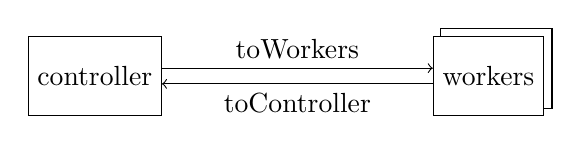
\begin{tikzpicture}
\draw (0,0) node[draw, minimum height = 10mm](c){\scalashape controller};
\draw (5,0) node[draw, minimum height = 10mm] (w){\scalashape workers};
\draw ([xshift = 1mm] w.north west) -- ++ (0,1mm) -- 
  ([xshift = 1mm, yshift = 1mm] w.north east) -- 
  ([xshift = 1mm, yshift = 1mm] w.south east) -- 
  ([yshift = 1mm] w.south east) ;
\draw[->] ([yshift = 1mm] c.east) -- node[above]{\scalashape toWorkers} 
  ([yshift = 1mm] w.west);
\draw[<-] ([yshift = -1mm] c.east) -- node[below]{\scalashape toController} 
  ([yshift = -1mm] w.west);
\end{tikzpicture}
\end{center}

In examples so far, each channel has had one sender and one receiver.  But an
inport or outport may be shared between any number of receivers or senders.
\end{slide}

%%%%%

%% \begin{slide}
%% \heading{Shared channels in CSO}

%% So far our channels have connected \emph{one} sender with \emph{one}
%% receiver.  But there are several other options.
%% %
%% \begin{itemize}
%% \item 
%% |N2N[T](writers, readers)| gives a channel intended to be used by |writers|
%% senders and |readers| receivers;

%% \item |OneMany[T]| gives a channel intended to be used by one sender and any
%% number of receivers;

%% \item |ManyOne[T]| gives a channel intended to be used by any number of
%% senders and one receiver.
%% \end{itemize}

%%%%%

%% \begin{slide}
%% \heading{Shared channels in CSO}

%% A compiler cannot \textit{completely} enforce the restrictions on sharing.
%% Infractions may even go undetected dynamically (though the code is cautious).
%% This is the responsibility of the programmer. 

%% An |N2N[T](writers, readers)| channel can be closed by |writers| senders
%% calling |closeOut|, or |readers| receivers calling |closeIn|.  A |OneMany[T]|
%% channel can be closed by the sender calling |closeOut|, but cannot be closed
%% by the receivers.  Likewise for  |ManyOne[T]| channels.
%% \end{slide}

%%%%%

\begin{slide}
\heading{Defining the channels}  

We want to experiment to see whether using buffered channels is advantageous.
So define
\begin{scala}
  private def mkChan[A: scala.reflect.ClassTag]: Chan[A] = 
    if(buffering > 0) new BuffChan[A](buffering) else new SyncChan[A]
\end{scala}

The controller needs to tell each worker the range \SCALA{[l,r]} to work on,
the number \SCALA{taskSize} of intervals in its range, and the size
\SCALA{delta} of each interval (so $\sm{taskSize} \times \sm{delta} \approx
\sm{r} - \sm{l}$).

We can pass this as a 4-tuple \SCALA{(l, r, taskSize, delta)}, so define:
%
\begin{scala}
  private type Task = (Double, Double, Int, Double)
  private val toWorkers = mkChan[Task]
\end{scala}

Each worker returns a \SCALA{Double} to the controller so define:
%
\begin{scala}
  private val toController = mkChan[Double]
\end{scala}
\end{slide}

%%%%%

\begin{slide}
\heading{A worker}

\begin{scala}
  /** A worker, which receives arguments from the controller, estimates the
    * integral, and returns the results. */
  private def worker = thread("worker"){
    val (left, right, taskSize, delta) = toWorkers?()
    val result = integral(left, right, taskSize, delta)
    toController!result
  }
\end{scala}
\end{slide}  

%%%%%

\begin{slide}
\heading{The controller}

For simplicity, we will assume that \SCALA{n} (the number of intervals) is
divisible by \SCALA{nWorkers} (the number of workers).  (The code on the
website avoids this assumption.) 

So each worker receives a task containing \SCALA{taskSize = n/nWorkers}
intervals, each of size \SCALA{delta = (b-a)/n}, i.e.~a range of size
\SCALA{taskRange = (b-a)/nWorkers}.

% containing \SCALA{taskSize = n/nWorkers} intervals, each of size \SCALA{delta =
%   (b-a)/n}. 

For convenience, the controller uses an object variable to store the result. 
\begin{scala}
  /** This variable ends up holding the result. */
  private var result = 0.0
\end{scala}
\end{slide}

%%%%%

\begin{slide}
\heading{The controller}

\begin{scala}
  /** A controller, who distributes tasks to the clients, and accumulates the
    * sub-results into result. */
  private def controller = thread("controller"){
    val delta = (b-a)/n
    val taskSize = n/nWorkers
    val taskRange = (b-a)/nWorkers
    var left = a // left hand boundary of next task
    for(i <- 0 until nWorkers){
      val right = left+taskRange
      toWorkers!(left, right, taskSize, delta)
      left = right
    }

    // Receive results, and add them up
    result = 0.0
    for(i <- 0 until nWorkers) result += (toController?())
  }    
\end{scala}
\end{slide}

%%%%%

\begin{slide}
\heading{Putting the system together}

\begin{scala}  
class Trapezium(f: Double => Double, a: Double, b: Double, 
  n: Long, nWorkers: Int, buffering: Int = 0)
    extends TrapeziumT(f, a, b){
  require(n >= nWorkers && n%nWorkers == 0)
  ...
  
  /** The main system. */
  private def system = {
    val workers = || (for (i <- 0 until nWorkers) yield worker)
    workers || controller
  }

  /** Calculate the integral, and return the result. */
  def apply: Double = { run(system); result } 
}
\end{scala}
\end{slide}

%%%%%

%% \begin{slide}
%% \heading{Testing}

%% How can we test the correctness of the concurrent program?
%% \end{slide}

%%%%%

\begin{slide}
\heading{Testing}

We could run the sequential and concurrent implementations on the same
integral, and test whether they give the same result.  (This assumes the
sequential implementation is correct.)   

If we use both implementations to estimate $\int_0^3 x^2 \mbox{d}x$ using
$100$ intervals, the sequential algorithm always gives
\begin{scala}
  9.000449999999995
\end{scala}
%
and the concurrent implementation with 10 workers gives
\begin{scala}
  9.000449999999999
  9.000449999999997
  9.000449999999999
  9.000449999999999
  9.000449999999997 
\end{scala}
on five successive runs.
How can we explain this?
\end{slide}

%%%%%

\begin{selfnote}
\heading{Numerical errors}

The difference in results on the previous slide can be explained by rounding
errors, and in particular that machine addition is not associative.  From the
Scala interpreter:
\begin{scala}
scala> (1E10 + (-1E10)) + 1E-10
res0: Double = 1.0E-10

scala> 1E10 + (-1E10 + 1E-10)
res1: Double = 0.0
\end{scala}
%
In the sequential algorithm, the values for the intervals are added up from
left to right.  But in the concurrent algorithm, they are added up in a
different order, giving a different result. 

In different runs of the concurrent algorithm, the sub-results are returned to
the controller in different orders, and so added up in different orders,
giving different results. 
\end{selfnote}

%%%%%

\begin{slide}
\heading{Testing}

My approach is:
%
\begin{enumerate}
\item Pick random values for |f| (I use random polynomials), |a|, |b|, |n| and
|nWorkers| (obeying the relevant preconditions);

\item Use both implementations to calculate the integral;

\item Test whether the results are approximately equal; I use
\begin{scala}
assert(
  seqResult != 0.0 && Math.abs((seqResult-concResult)/seqResult) < 1E-7 ||
    Math.abs(seqResult-concResult) < 1E-10, ...)
\end{scala}

\item Repeat a few million times.
\end{enumerate}
\end{slide}

%%%%%

\begin{selfnote}
When I tried this, I found various bugs indicating that I hadn't thought
carefully enough about the preconditions, for example that |n >= nWorkers|.

I initially just looked at the relative error, which failed in a case where
|seqResult| and |concResult| were both very small, and the relative error was
about one part in $10^6$.  

More interestingly, I found a deadlock within the CSO code for the channel.
\end{selfnote}
